\documentclass[12pt]{article}
\usepackage{graphicx} % Required for inserting images

\usepackage{cite}
\usepackage{amsmath}
\usepackage{circuitikz}
\usepackage{booktabs}
\usepackage{siunitx}
\usepackage{afterpage}
\usepackage{amsmath,amssymb,amsfonts}
\usepackage{algorithmic}
\usepackage{graphicx}
\usepackage{textcomp}
\usepackage{xcolor}
\usepackage{amssymb}
\usepackage{siunitx}
\usepackage{float}
\PassOptionsToPackage{hyphens}{url}\usepackage{hyperref}
\usepackage{cleveref}
\usepackage[utf8]{inputenc}
\usepackage[right]{lineno}
\usepackage{csquotes}
\usepackage{booktabs}
\usepackage{longtable}
\usepackage{adjustbox}
\usepackage{titlesec}
\usepackage{tikz,xcolor,pgfplots}
\usepackage{amsthm}
\theoremstyle{definition}
\newtheorem{example}{Ejemplo}

\usepackage{setspace}          % Espaciado personalizado
\usepackage{amsmath, amssymb}  % Símbolos matemáticos
\usepackage{tcolorbox}         % Recuadros de color
\usepackage{tikz}              % Diagramas de bloque
\usepackage{geometry}          % Márgenes
\usepackage{fancyhdr}          %Encabezados y pie de página
\usepackage{xcolor}



%Paquetes
\usepackage[utf8]{inputenc}
\usepackage[T1]{fontenc}
\usepackage[spanish]{babel}
\usepackage{geometry}
\usepackage{fancyhdr}
\usepackage{titlesec}
\usepackage{hyperref}
\usepackage{framed}
\usepackage{graphicx}

\title{Cap 6.4_6.5}
\author{ARTURO RUIZ TARAZONA}
\date{September 2025}


%Márgenes
\geometry{
  top=2.5cm,
  bottom=2.5cm,
  left=2.5cm,
  right=2.5cm
}

%Hipervínculos azules
\hypersetup{
  colorlinks=true,
  linkcolor=blue,
  urlcolor=blue,
  citecolor=blue
}

%Encabezado/Pie
\pagestyle{fancy}
\fancyhf{} % limpiar

% Texto del encabezado (izquierda, en cursiva, tamaño reducido)
\newcommand{\encabezadoSuperior}{6.4. MODELOS TEMPORIZADOS DE COMPUTACIÓN}
\fancyhead[L]{\small\itshape\encabezadoSuperior}

% Número de página al costado (abajo-izquierda)
\fancyfoot[L]{\thepage}

% Descripción azul en el pie (abajo-derecha)
\newcommand{\pieAzul}{Lee \& Seshia, \textit{Introducción a los Sistemas Embebidos}}
\fancyfoot[R]{\textcolor{blue}{\pieAzul}}

% Línea horizontal bajo el encabezado
\renewcommand{\headrulewidth}{0pt}  % desactiva la regla por defecto
\makeatletter
\renewcommand{\headrule}{%
  \hrule \@height 0.4pt \@width \paperwidth \vskip0pt%
}
\makeatother

% Formato de títulos
\titleformat{\section}{\bfseries\Large}{}{0pt}{}
\titleformat{\subsection}{\bfseries\large}{}{0pt}{}



\usetikzlibrary{arrows.meta, positioning,shapes.geometric} 

\geometry{margin=3cm}
\setstretch{1.4}
\setlength{\parskip}{4pt} 
\pagestyle{empty}

\thispagestyle{fancy}
\fancyhf{} 
\fancyhead[L]{\textit{\textcolor{black}{2.2 MODELO DE ACTORES}}}
\fancyfoot[R]{\textcolor{blue}{\textit{Lee \& Seshia, Introducción a los Sistemas Embebidos}}} 
\fancyfoot[L]{24}
\tcbset{
    colback=cyan!10,
    colframe=cyan!50!black, 
    boxrule=0.8pt,
    arc=3pt,
    left=6pt,
    right=6pt,
    top=6pt,
    bottom=6pt
}

\usepackage{mdframed}
\usepackage[utf8]{inputenc}
\usepackage[spanish]{babel}
\usepackage{xcolor}
\usepackage{amsmath, amssymb}
\usepackage{tcolorbox}
\tcbset{
    colback=cyan!10, % Fondo celeste suave
    colframe=cyan!50!black, % Borde más oscuro
    boxrule=0.8pt,
    arc=3pt,
    left=6pt,
    right=6pt,
    top=6pt,
    bottom=6pt
}


\title{PC1 - Tarea 1 -  Latex 25-2}
\author{segundo }
\date{August 2025}

\begin{document}

\maketitle



\section{Sistemas Hibridos}

Los capítulos 2 y 3 describen dos estrategias de modelado muy diferentes, una centrada en la dinámica continua y otra en la dinámica discreta. Para la dinámica continua, utilizamos ecuaciones diferenciales y sus correspondientes modelos de actores. Para la dinámica discreta, utilizamos máquinas de estados.
\ \ \\
Los sistemas ciberfísicos integran la dinámica física y los sistemas computacionales, por lo que comúnmente combinan dinámicas discretas y continuas. En este capítulo, mostramos que las técnicas de modelado de los capítulos 2 y 3 se pueden combinar, dando lugar a lo que se conoce como sistemas híbridos. Los modelos de sistemas híbridos suelen ser mucho más simples y comprensibles que los modelos de fuerza bruta que se limitan a solo uno de los dos estilos de los capítulos 2 y 3. Son una herramienta poderosa para comprender los sistemas del mundo real.

\subsection{Modelos modales}

En esta sección, mostramos que las máquinas de estados se pueden generalizar para admitir entradas y salidas continuas y para combinar dinámicas discretas y continuas.

\subsubsection{Modelo de actor para máquinas de estados}

En la Sección 3.3.1 explicamos que las máquinas de estados tienen entradas definidas por el conjunto \textit{Entradas} que pueden ser señales puras o pueden llevar un valor. En cualquier caso, la máquina de estados tiene varios puertos de entrada, que en el caso de las señales puras están presentes o ausentes, y en el caso de las señales con valor tienen un valor en cada reacción de la máquina de estados.

También explicamos en la Sección 3.3.1 que las acciones en las transiciones establecen los valores de las salidas. Las salidas también se pueden representar por puertos, y nuevamente los puertos pueden llevar señales puras o señales con valor. En el caso de las señales puras, una transición que se toma especifica si la salida está presente o ausente, y en el caso de las señales con valor, asigna un valor o afirma que la señal está ausente. Se presume que las salidas están ausentes entre transiciones.

Dada esta visión de entrada/salida de las máquinas de estados, es natural pensar en una máquina de estados como un actor, como se ilustra en la Figura 4.1. En esa figura, asumimos un número $n$ de puertos de entrada llamados $I1$. En cada reacción, estos puertos tienen un valor que está presente o ausente (si el puerto transporta una señal pura) o es miembro de algún conjunto de valores (si el puerto transporta una señal con valor). Las salidas son similares. Las guardas en las transiciones definen subconjuntos de posibles valores en los puertos de entrada, y las acciones asignan valores a los puertos de salida. Dado tal modelo de actor, es sencillo generalizar las FSM para admitir señales de tiempo continuo como entradas.


\subsubsection{Entradas continuas}


Hasta ahora hemos asumido que las máquinas de estados operan en una secuencia de reacciones discretas.

Hemos asumido que no hay entradas ni salidas entre reacciones. Ahora generalizaremos esto para permitir que 
\textcolor{blue}{
las entradas y las salidas sean señales de tiempo continuo.
}



    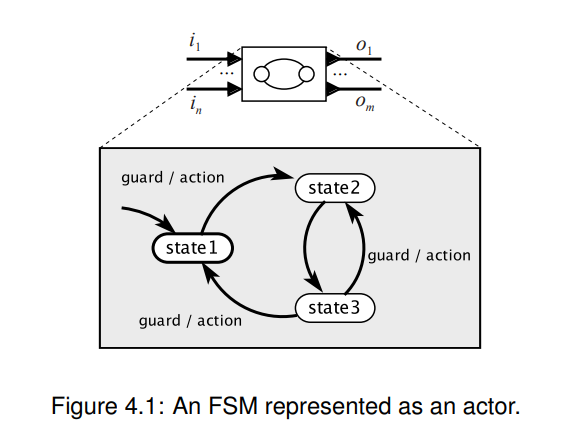
\includegraphics[width=0.5\linewidth]{4_4.1/fig4.png}
    
Para que los modelos de maquina de estados coexistan con los modelos basados en el tiempo, necesitamos interpretar que las transiciones de estado ocurren en la misma línea de tiempo utilizada para la parte temporal del sistema. El concepto de reacciones discretas descrito en la Sección 3.1 es suficiente para este propósito, pero ya no se requerirá que las entradas y salidas estén ausentes entre reacciones. En su lugar, definiremos que una transición ocurre cuando se habilita una protección en una transición saliente desde el estado actual. Como antes, durante el tiempo entre reacciones, se entiende que una máquina de estados no realiza transiciones entre modos. Sin embargo, ya no se requiere que las entradas y salidas estén ausentes durante ese tiempo.

\begin{tcolorbox}
\textbf{Ejemplo 4.1:} Considere un termostato modelado como una máquina de estados con estados 
\(\Sigma = \{\text{calentamiento}, \text{enfriamiento}\}\), como se muestra en la Figura 4.2. 
Esta es una variante del modelo del Ejemplo 3.5, donde, en lugar de una entrada discreta que proporciona una 
temperatura en cada reacción, la entrada es una señal continua 
\(\tau: \mathbb{R} \to \mathbb{R}\), donde \(\tau(t)\) representa la temperatura en el tiempo \(t\).  

El estado inicial es enfriamiento, y la transición para salir de este estado se habilita en el tiempo \(t\) más 
temprano después del tiempo de inicio, cuando \(\tau(t) \leq 18\).  

En este ejemplo, asumimos que las salidas son señales puras de calor activado y calor desactivado.

\end{tcolorbox}

En el ejemplo anterior, las salidas solo están presentes en los momentos en que se toman las transiciones. 
También podemos generalizar las FSM para que admitan salidas de tiempo continuo, pero para ello, necesitamos 
la noción de refinamientos de estado.  

\subsubsection*{4.1.3 Refinamientos de estado}

\text{Un sistema híbrido asocia con cada estado de una FSM un comportamiento dinámico. Nuestro primer ejemplo 
(muy simple) utiliza esta capacidad simplemente para producir salidas de tiempo continuo.}

\begin{tcolorbox}
    Ejemplo 4.2: Supongamos que, en lugar de salidas discretas como en el Ejemplo 4.1, deseamos generar una señal de control cuyo valor sea 1 cuando la calefacción esté encendida y 0 cuando esté apagada. Dicha señal de control podría controlar directamente un calefactor. El termostato de la Figura 4.3 lo hace. En dicha figura, cada estado tiene un refinamiento que proporciona el valor de la salida h mientras la máquina de estados se encuentra en ese estado.
\end{tcolorbox}
En un sistema híbrido, el estado actual de la máquina de estados tiene un refinamiento de estado que proporciona el comportamiento dinámico de la salida en función de la entrada. En el ejemplo simple anterior, la salida es constante en cada estado, lo cual es una dinámica bastante trivial. Los sistemas híbridos pueden ser mucho más elaborados.

La estructura general de un modelo de sistema híbrido se muestra en la Figura 4.4. En esa figura, hay una máquina de estados finitos de dos estados. Cada estado está asociado con un refinamiento de estado

\begin{figure}[H]
    \centering
    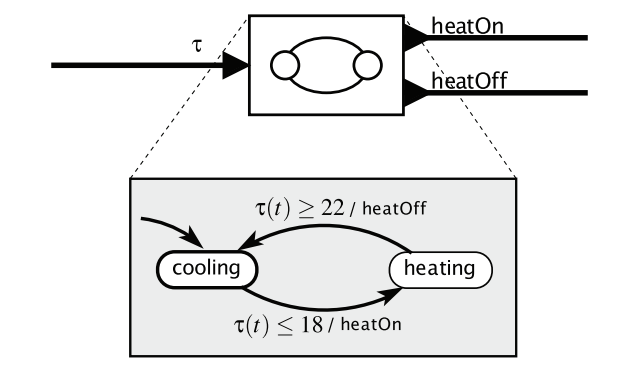
\includegraphics[width=0.5\linewidth]{4_4.1/image.png}

    \caption{Un termostato modelado como un FSM con una señal de entrada de tiempo continuo.}
    \label{Figura 4.2}
\end{figure}

Etiquetado en la figura como un "sistema basado en el tiempo". El refinamiento de estado define el comportamiento dinámico de las salidas y (posiblemente) variables de estado continuas adicionales. Además, cada transición puede especificar opcionalmente acciones establecidas, que establecen los valores de dichas variables de estado adicionales cuando se realiza una transición. El ejemplo de la Figura 4.3 es bastante simple, ya que no tiene variables de estado continuas, ni acciones de salida, ni acciones establecidas.

Un sistema híbrido a veces se denomina modelo modal porque tiene un número finito de modos, uno para cada estado de la FSM, y cuando está en un modo, su dinámica se especifica mediante el refinamiento de estado. Los estados de la FSM pueden denominarse modos en lugar de estados, lo que, como veremos, ayuda a evitar confusiones con los estados de los refinamientos.

La siguiente dinámica más simple, además de las salidas constantes bastante triviales del Ejemplo 4.2, se encuentra en los autómatas temporizados, que analizamos a continuación.



\end{document}
